\documentclass{article}
\usepackage[english,russian]{babel}
\usepackage{textcomp}
\usepackage{geometry}
  \geometry{left=2cm}
  \geometry{right=1.5cm}
  \geometry{top=1.5cm}
  \geometry{bottom=2cm}
\usepackage{tikz}
\usepackage{multicol}
\usepackage{hyperref}
\usepackage{listings}
\usepackage{pmboxdraw}
\usepackage{fancyvrb}
\usepackage{lipsum}
\usepackage[shortlabels]{enumitem}
\pagenumbering{gobble}

\lstdefinestyle{csMiptCppStyle}{
  language=C++,
  basicstyle=\linespread{1.1}\ttfamily,
  columns=fixed,
  fontadjust=true,
  basewidth=0.5em,
  keywordstyle=\color{blue}\bfseries,
  commentstyle=\color{gray},
  texcl=true,
  stringstyle=\ttfamily\color{orange!50!black},
  showstringspaces=false,
  numbersep=5pt,
  numberstyle=\tiny\color{black},
  numberfirstline=true,
  stepnumber=1,      
  numbersep=10pt,
  backgroundcolor=\color{white},
  showstringspaces=false,
  captionpos=b,
  breaklines=true
  breakatwhitespace=true,
  xleftmargin=.2in,
  extendedchars=\true,
  keepspaces = true,
  tabsize=4,
  upquote=true,
}


\lstdefinestyle{csMiptCppLinesStyle}{
  style=csMiptCppStyle,
  frame=lines,
}

\lstdefinestyle{csMiptCppBorderStyle}{
  style=csMiptCppStyle,
  framexleftmargin=5mm, 
  frame=shadowbox, 
  rulesepcolor=\color{gray}
}


\lstdefinestyle{csMiptBash}{
  	style=csMiptCppStyle,
	breaklines=true,
	frame=tb,
	language=bash,
	breakatwhitespace=true,
	alsoletter={*()"'0123456789.},
	alsoother={\{\=\}},
	basicstyle={\ttfamily},
	keywordstyle={\bfseries},
	literate={{=}{{{=}}}1},
	prebreak={\textbackslash},
	sensitive=true,
	stepnumber=1,
	tabsize=4,
	morekeywords={echo, function},
	otherkeywords={-, \{, \}},
	literate={\$\{}{{{{\bfseries{}\$\{}}}}2,
	upquote=true,
	frame=none
}

\lstset{style=csMiptBash}
\lstset{
        literate={~}{{\raisebox{0.5ex}{\texttildelow}}}{1}
}

\renewcommand{\thesubsection}{\arabic{subsection}}
\makeatletter
\def\@seccntformat#1{\@ifundefined{#1@cntformat}%
   {\csname the#1\endcsname\quad}
   {\csname #1@cntformat\endcsname}}
\newcommand\section@cntformat{}     
\newcommand\subsection@cntformat{Задача \thesubsection.\space} 
\newcommand\subsubsection@cntformat{\thesubsubsection.\space}
\makeatother



\begin{document}
\title{Семинар \#3: git, продвинутый. Практика. \vspace{-5ex}}\date{}\maketitle

\subsection*{Как сдавать задачи}
Для сдачи ДЗ вам нужно создать репозиторий на GitLab (если он ещё не создан) под названием \texttt{devtools-homework}. Структура репозитория должна иметь вид:
\begin{center}
\begin{BVerbatim}
├── seminar3_advanced_git/
│   ├── 01.sh
│   ├── 02.sh
│   ├── 03.sh
│   └── ...
└── ...
\end{BVerbatim}
\end{center}
Для каждой задачи, если не сказано иное, нужно создать 1 файл решения с расширением \texttt{.sh}. Для каждой подзадачи нужно прописать все команды, которые исполняются в ходе выполнения этой подзадачи. Оформлять файл решения нужно в следующем формате:
\begin{lstlisting}
# Subtask a
git merge feature
# Конфликт, разрешаю вручную
git add имена файлов
git merge --continue
# Открылся редактор, ввожу:
# This is my merge commit!

# Subtask b
git reset --hard HEAD~2
# Открываю reflog и ищу нужный коммит
git reset --hard 24e1f51
...
\end{lstlisting}
Если в задаче встречается вопрос или требование, то на это нужно ответить в комментариях (\texttt{\#}) файла решения. 




\subsection{Диапазоны}
\subsubsection*{Подготовка: генерация репозитория}
\begin{minipage}[t]{0.55\linewidth}
\vspace*{0mm}
Для решения этой задачи вам понадобится сгенерировать репозиторий с помощью скрипта \texttt{create\_two\_branch\_repo.sh}, который можно найти в папке: \href{https://mipt-hsse.gitlab.yandexcloud.net/v.biryukov/devtools_course/-/tree/main/seminar3_advanced_git/practice/scripts}{\texttt{seminar3\_advanced\_git/practice/scripts}}. Для этого нужно проделать следующие шаги:
\begin{enumerate}
\item Скачайте скрипт к себе на компьютер
\item Сделайте скрипт исполняемым:
\begin{lstlisting}
$ chmod +x ./create_two_branch_repo.sh
\end{lstlisting}
\vspace{-2mm}
\item Запустите его:
\begin{lstlisting}
$ ./create_two_branch_repo.sh test
\end{lstlisting}
\vspace{-2mm}
\item В результате сгенерируется директория \texttt{test} с репозиторием. Зайдите в эту директорию и выполните:
\begin{lstlisting}
$ git log --oneline --all --graph
\end{lstlisting}
\vspace{-2mm}
чтобы убедиться, что граф репозитория совпадает с тем, что изображено на рисунке.
\end{enumerate}

\end{minipage}
\hfill
\begin{minipage}[t]{0.40\linewidth}
\vspace*{0mm}
\includegraphics[width=0.95\textwidth]{../images/00two_branch_animals.pdf}
\end{minipage}

\subsubsection*{Подзадачи}
\textbf{Важно!} В файле решения, в комментариях, выпишите результат выполнения всех команд этой задачи. Это важно, так как хэши коммитов в вашем репозитории могут отличаться (так как репозиторий генерируется скриптом), и я не смогу проверить задание, не зная хешей коммитов в вашем репозитории. 

Также, во всех подзадачах это задачи нужно выполнить задание без явного перечисления все коммитов. В реальных проектах в одной ветке могут быть тысячи коммитов и перечислить их всех не получится.

\begin{enumerate}[a.]
\item \textbf{Хэши всех коммитов}\\
Выполните команду, которая будет печатать для каждого коммита в репозитории только его сокращённый хэш и его сообщение в следующем формате. 
\begin{lstlisting}
Hash: 5b58166, message: "CF: add fox in animals.txt"
Hash: 5838367, message: "CD: add dog in animals.txt"
Hash: b25757f, message: "CE: add emu in animals.txt"
Hash: 7e58924, message: "CC: add cat in animals.txt"
Hash: 6f928eb, message: "CB: add bat in animals.txt"
Hash: a353350, message: "CA: add axolotl in animals.txt"
Hash: eca0dc3, message: "C0: initial commit"
\end{lstlisting}


\item \textbf{Диапазон коммитов, достижимых от одной ветки}\\
Выполните команду, которая будет печатать хэши всех коммитов, достижимых от ветки \texttt{feature}.

\item \textbf{Разность множеств коммитов двух веток}\\
Пусть $S_{main}$ -- это множество всех коммитов, достижимых от ветки \texttt{main}, а $S_{feature}$ -- это множество всех коммитов, достижимых от ветки \texttt{feature}. Выполните команду, которая будет печатать хэши всех коммитов, принадлежащих $S_{feature} \setminus S_{main}$. То есть нужно напечатать хэши всех коммитов, достижимых из ветки \texttt{feature}, но не достижимых из ветки \texttt{main}. Решите эту подзадачу двумя способами:
\begin{enumerate}
\item Используя синтаксис с двумя точками
\item Используя синтаксис исключения коммитов с символом \texttt{$\wedge$}
\end{enumerate} 


\item \textbf{Симметрическая разность множеств коммитов двух веток}\\
Выполните команду, которая будет печатать хэши всех коммитов, принадлежащих симметрической разности двух множеств: $S_{main}\, \triangle\, S_{feature}$.

\item \textbf{Последние коммиты}\\
Используйте диапазон, чтобы напечатать хэши последних трёх коммитов в ветке \texttt{main}.

\item \textbf{Общий предок двух веток}\\
Выполните команду, которая будет печатать хэш ближайшего общего предка веток \texttt{main} и \texttt{feature}.


\item \textbf{Разница между двумя коммитами}\\
Выведите разницу между коммитами \texttt{main} и \texttt{main$\sim$}, используя команду:
\begin{lstlisting}
$ git diff main main~
\end{lstlisting}
Объясните, что означает каждая строка данного вывода.

\item \textbf{Разница между ветками}\\
Выведите разницу между ветками \texttt{main} и \texttt{feature}. Обратите внимание, что синтаксис перечисления коммитов через две/три точки имеет другое значение в команде \texttt{git diff} по сравнению со всеми другими командами \texttt{git}. Решите эту задачу двумя способами:
\begin{enumerate}
\item Передав \texttt{git diff} имена веток через аргументы.
\item Используя синтаксис \texttt{git diff A..B} (две точки).
\end{enumerate}


\item \textbf{Разница между веткой и общим предком}\\
Выведите разницу между веткой \texttt{feature} и общим предком этой ветки с веткой \texttt{main}. Решите эту задачу двумя способами:
\begin{enumerate}
\item Используя команду \texttt{git merge-base}.
\item Используя синтаксис \texttt{git diff A...B} (три точки).
\end{enumerate}

\end{enumerate}



\subsection{Типы слияния}
\begin{enumerate}[a.]
\item \textbf{Трехстороннее слияние (слияние по умолчанию)}\\
Самый распространённый тип слияния, при котором git ищет общего предка двух веток и смотрит на:
\vspace{-2mm}
\begin{enumerate}[(A)]
\item Общий предок (\texttt{merge-base})
\item Текущая ветка (\texttt{HEAD})
\item Сливаемая ветка (\texttt{feature})
\end{enumerate}
\vspace{-2mm}
Git попытается объединить изменения из B и C относительно общего предка A. Если строки изменены в обеих ветках, возникает конфликт, который нужно разрешить вручную.
\begin{center}
\includegraphics[width=0.6\linewidth]{../images/01three_way_merge.pdf}
\end{center}
Сгенерируйте новый репозиторий с помощью скрипта \texttt{create\_two\_branch\_repo.sh} и сделайте слияние ветки \texttt{feature} в ветку \texttt{main}, используя трёхстороннее слияние. Что будет содержаться в файле \texttt{animals.txt} до разрешения конфликта? Разрешите конфликт и создайте коммит слияния \texttt{CM}.

\item \textbf{Трехстороннее слияние с опциями \texttt{ours} и \texttt{theirs}}\\
Снова создайте репозиторий через \texttt{create\_two\_branch\_repo.sh}. Сделайте слияние \texttt{feature} в \texttt{main}, используя трёхстороннее слияние с опцией \texttt{ours}. Снова сгенерируйте новый репозиторий и сделайте слияние, используя опцию \texttt{theirs}. Что будет содержаться в \texttt{animals.txt} после каждого из слияний?

\item \textbf{Squash-слияние (хотя технически это не слияние)}\\
Squash-слияние -- это способ объединить все изменения другой ветки в один коммит текущей ветки.
\begin{center}
\includegraphics[width=0.6\linewidth]{../images/02squash_merge.pdf}
\end{center}
Сгенерируйте новый репозиторий с помощью скрипта \texttt{create\_two\_branch\_repo.sh} и сделайте squash-слияние ветки \texttt{feature} в ветку \texttt{main}.

\item \textbf{Сливаемая ветка позади текущей}\\
\begin{minipage}[t]{0.55\linewidth}
\vspace*{0mm}
Предположим, что ветка \texttt{feature} находится позади ветки \texttt{main} и мы пытаемся сделать слияние \texttt{feature} в \texttt{main}:
\begin{lstlisting}
$ git switch main
$ git merge feature
\end{lstlisting}
Ответь на следующие вопросы:
\begin{enumerate}
\item Будет ли создан новый коммит (коммит слияния) при такой операции?
\item Куда будет указывать ветка \texttt{main}?
\item Куда будет указывать ветка \texttt{feature}?
\end{enumerate}
Сгенерировать репозиторий можно с помощью скрипта \texttt{create\_feature\_behind\_main.sh}, который можно найти в \href{https://mipt-hsse.gitlab.yandexcloud.net/v.biryukov/devtools_course/-/tree/main/seminar3_advanced_git/practice/scripts}{\texttt{seminar3\_advanced\_git/practice/scripts}}.
\end{minipage}
\hfill
\begin{minipage}[t]{0.4\linewidth}
\vspace*{0mm}
\begin{center}
\includegraphics[width=0.55\linewidth]{../images/03feature_behind_main.pdf}
\end{center}
\end{minipage}
\item \textbf{Сливаемая ветка впереди текущей: слияние перемоткой}\\
Предположим, что ветка \texttt{feature} находится впереди ветки \texttt{main} и мы хотим сделать слияние перемоткой ветки \texttt{feature} в ветку \texttt{main}:
\begin{center}
\includegraphics[width=0.55\linewidth]{../images/05feature_ahead_ff.pdf}
\end{center}
Сгенерируйте репозиторий с помощью скрипта \texttt{create\_feature\_ahead\_main.sh} и произведите слияние перемоткой ветки \texttt{feature} в ветку \texttt{main}.

\item \textbf{Сливаемая ветка впереди текущей: слияние без перемотки}\\
\begin{center}
\hspace{1.65cm}\includegraphics[width=0.65\linewidth]{../images/06feature_ahead_no_ff.pdf}
\end{center}
Снова сгенерируйте репозиторий с помощью скрипта \texttt{create\_feature\_ahead\_main.sh} и произведите обычное слияние без перемотки ветки \texttt{feature} в ветку \texttt{main}.

\item \textbf{Octopus-слияние}\\
Git поддерживает слияние сразу нескольких веток одной операцией, но только с условием, что при этом не произойдёт ни одного конфликта. Это так называемое octopus-слияние.
\begin{center}
\includegraphics[width=0.5\linewidth]{../images/07octopus.pdf}
\end{center}
Сгенерируйте репозиторий с помощью скрипта \texttt{create\_octopus.sh} и произведите слияние веток \texttt{alice}, \texttt{bob}, \texttt{casper} и \texttt{diana} в ветку \texttt{main}. Распечатайте хэши всех родителей получившегося коммита слияния, используя \texttt{$\wedge$}-нотацию и команду \texttt{git rev-parse}.


\end{enumerate}
\subsection{Работа с репозиторием}



\subsubsection*{Подготовка. Генерация репозитория, который будет использоваться в подзадачах}
Репозиторий для этой задачи можно найти по адресу:
\href{https://mipt-hsse.gitlab.yandexcloud.net/v.biryukov/utils}{\texttt{mipt-hsse.gitlab.yandexcloud.net/v.biryukov/utils}}. Клонируйте этот репозиторий себе:
\begin{lstlisting}
git clone git@mipt-hsse.gitlab.yandexcloud.net:v.biryukov/utils.git
cd utils
\end{lstlisting}
\subsubsection*{Подзадачи}
\begin{enumerate}[a.]
\item \textbf{Просмотр содержимого репозитория}\\
Перейдите на все ветки и посмотрите, какие файлы содержатся в их последних коммитах:
\begin{lstlisting}
$ git switch alice
$ git switch bob
$ git switch main
\end{lstlisting}
Это важно сделать ещё и потому, что при клонировании репозитория создаются только remote-tracking ветки (например, \texttt{origin/alice}), тогда как обычные локальные ветки (например, \texttt{alice}) отсутствуют. Их можно создать вручную или же они будут созданы автоматически при переключении на них -- при условии, что соответствующая remote-tracking ветка существует.

\item \textbf{Просмотрите граф коммитов}\\
Это можно сделать на GitLab во вкладке \texttt{Code -> Repository Graph} или у вас на машине, с помощью:
\begin{lstlisting}
$ git log --oneline --all --graph
\end{lstlisting}
Для вывода на экран, если вывод не помещается на экран полностью, команда \texttt{git log} используется программу \texttt{less}. Чтобы показать следующую строчку используйте \texttt{Enter}. Чтобы выйти из программы \texttt{less} просто нажмите клавишу \texttt{Q}.

\iffalse
В этом выводе будут отображаться как обычные ветки (вроде \texttt{alice}), так и удалённые ветки (вроде \texttt{origin/alice}). Чтобы удалённые ветки не отображались будем использовать следующую команду:
\begin{lstlisting}
$ git log --oneline --all --graph --decorate-refs-exclude=refs/remotes/*
\end{lstlisting}
\fi

\item \textbf{Новый alias}\\
Добавьте новый \texttt{alias} для этой команды, назовите его \texttt{lg}. То есть теперь, при вызове: 
\begin{lstlisting}
$ git lg
\end{lstlisting}
Должно печататься то же, что и при вызове 
\begin{lstlisting}
$ git log --oneline --all --graph
\end{lstlisting}

\item \textbf{Повторное использование записанного разрешения конфликта}\\
В процессе работы с большими репозиториями могут возникнуть ситуации, когда один и тот же конфликт приходится разрешать множество раз. Git может самостоятельно разрешать повторяющиеся конфликты, если включить специальную опцию \texttt{rerere} (\textit{reuse recorded resolution}). Включите эту опцию локально для данного репозитория.


\item \textbf{Слияние с конфликтом}\\
Слейте ветку \texttt{bob} в ветку \texttt{main}. Для этого вам нужно перейти в ветку \texttt{main} и вызвать:
\begin{lstlisting}
$ git merge bob
\end{lstlisting}
При этом должен возникнуть конфликт. Разрешите его. Если у вас включена настройка \texttt{rerere}, то Git запомнит то, как вы разрешили этот конфликт. В этой и последующих задачах необязательно, чтобы код после слияния был корректным, так как это задание на git, а не на язык программирования. Посмотрите как выглядит граф коммитов после слияния с помощью \texttt{git lg}.

\item \textbf{Отмена слияния и повторное разрешение конфликта}\\
Отмените только что выполненное слияние. Затем произведите слияние заново. На этот раз конфликт должен разрешиться автоматические. Вам нужно будет только проверить результат и создать коммит слияния.

\item \textbf{Отмена слияния}\\
Отмените только что выполненное слияние, используя \texttt{ORIG\_HEAD} или \texttt{HEAD@\{1\}}.

\item \textbf{Перебазирование с конфликтом}\\
Перебазируйте ветку \texttt{bob} на ветку \texttt{main}. Для этого вам нужно перейти в ветку \texttt{bob} и вызвать:
\begin{lstlisting}
$ git rebase main
\end{lstlisting}
При этом могут возникнуть конфликты. Разрешите их. Посмотрите как выглядит граф коммитов после перебазирования с помощью \texttt{git lg}.

\item \textbf{Отмена перебазирования}\\
Отмените только что выполненное перебазирование, используя \texttt{ORIG\_HEAD} или \texttt{HEAD@\{1\}}.

\item \textbf{Копия диапазона коммитов с конфликтом}\\
Скопируйте из ветки \texttt{alice} на ветку \texttt{bob} диапазон коммитов от \texttt{4d6662c} до \texttt{fe2e890}, используя одну команду \texttt{git cherry-pick}. При этом могут возникнуть несколько конфликтов. Разрешите их. Посмотрите как выглядит граф коммитов с помощью \texttt{git lg}.


\item \textbf{Просмотр файлов}\\
Напишите команды, которые печатают файлы на экран:
\begin{itemize}
\item файл \texttt{arithmetic.py} из ветки \texttt{main}
\item файл \texttt{arithmetic.py} из коммита \texttt{alice$\sim$5}
\end{itemize}

\item \textbf{Разница}\\
Напишите команды, которые печатают на экран разницу (\texttt{diff}) между следующими коммитами или отдельными файлами:
\begin{itemize}
\item между коммитами \texttt{alice} и \texttt{alice$\sim$5}
\item между файлом \texttt{integration.py} в ветке \texttt{main} и файлом \texttt{integration.py} ветки \texttt{alice}.
\item между файлом \texttt{misc.py} коммита \texttt{fe2e890} и файлом \texttt{arithmetic.py} коммита \texttt{765df07}.
\end{itemize}


\item \textbf{Поиск первого коммита, содержащего ошибку}\\
Перейдите в ветку \texttt{alice} и запустите скрипт \texttt{sorting.py}
\begin{lstlisting}
python ./sorting.py
\end{lstlisting}
Вы увидите, что одна из сортировок работает неправильно, хотя в других ветках эта сортировка работала правильно. Значит в одном из коммитов ветки \texttt{alice} была допущена ошибка. Найдите коммит, в котором была допущена ошибка с помощью \texttt{git bisect}. Укажите в файле решения хэш коммита, файл и строчку в которой впервые возникает ошибка.

\item \textbf{\textbf{Фрагменты}}\\
Перейдите на ветку \texttt{alice} и добавьте изменения. В рабочей папке добавьте комментарии к функциям \texttt{add}, \texttt{factorial}, \texttt{is\_prime} и \texttt{is\_perfect\_number} из файла \texttt{arithmetic.py}. Комментарии должны выглядеть примерно так:
\vspace{-1mm}
\begin{lstlisting}[language=Python]
# This function adds two numbers
def add(a: float, b: float) -> float:
    return a + b
\end{lstlisting}
\vspace{-2mm}

Добавьте в индекс только изменения, связанные с функциями \texttt{add} и \texttt{is\_prime}. Остальные изменения добавлять не нужно. Создавать новый коммит не нужно. Используйте команду \texttt{git add} с опцией \texttt{-p}.



\item \textbf{\textbf{Хранилище}}\\
В реальной работе с репозиторием часто возникает следующая ситуация: вы работаете в какой-либо ветке, изменяете файлы, добавляете их в индекс, но пока не готовы делать коммит. В этот момент может возникнуть необходимость переключиться на другую ветку, например, чтобы срочно исправить баг. Если в рабочей директории или в индексе есть изменения которые могут быть перезаписаны при переключении на другую ветку, то Git не позволит выполнить \texttt{git switch}. Для решения этой проблемы можно использовать команду \texttt{git stash}, которая временно сохраняет изменения. После этого можно переключиться на другую ветку, выполнить нужную работу, а затем вернуться и восстановить сохранённые изменения.

После изменений, сделанных в прошлой подзадаче, попробуйте переключиться на ветку \texttt{main}. Произойдёт ошибка, так как есть несохранённые изменения в рабочей директории и в индексе. Используйте \texttt{git stash}, чтобы спрятать изменения. Перейдите на ветку \texttt{main} и сделайте там любой коммит. Вернитесь на ветку \texttt{alice} и восстановите изменения из \texttt{stash}. Восстановить изменения нужно таким образом, чтобы те изменения, которые были в индексе, остались в индексе, а те изменения, которые были в рабочей папке, остались в рабочей папке.

\item \textbf{Перенос хранилища}\\
Снова добавьте эти же изменения в \texttt{stash}. Перейдите на ветку \texttt{bob} и вытащите изменения, сделанные на ветке \texttt{alice}, в ветку \texttt{bob}. Возможен конфликт. Исправьте конфликт и сделайте коммит с этими изменениями в ветке \texttt{bob}.



\item \textbf{\textbf{Новая рабочая директория}}\\
Ещё один способ решения проблемы переключения на другую ветку при незакоммиченных изменениях -- это использование нескольких рабочих директорий, которые можно создать с помощью \texttt{git worktree}.

Перейдите в ветку \texttt{alice} и внесите изменения в рабочую директорию и индекс. После этого вы не сможете переключиться на ветку \texttt{bob}, используя \texttt{git switch}. Создайте новую рабочую директорию (\texttt{worktree}), соответствующую ветке \texttt{bob}. Лучше располагать её вне текущей рабочей директории, чтобы она не мешала работе над текущей веткой. Перейдите в новую рабочую директорию. Обратите внимание, что \texttt{.git} в этой директории является обычным файлом, а не директорией. Что содержится в этом файле? Сделайте любой коммит в ветке \texttt{bob} и вернитесь обратно в первоначальную рабочую директорию.

\iffalse
\item \textbf{Патч-файл}\\
Создайте патч-файл, содержащий изменения последних трёх коммитов ветки \texttt{alice}, используя \texttt{git diff}. Перейдите в ветку \texttt{main} и примените этот патч с помощью команды \texttt{git apply}. При этом могут возникнуть конфликты. Используйте команду \texttt{git apply} с опцией  \texttt{-{}-3way} для разрешения конфликтов. Сделайте коммит изменений, созданных патчем, в ветке \texttt{main}. Сам патч-файл удалите.
\fi

\item \textbf{Сборка мусора}\\
В этой задаче нужно полностью удалить коммит из локального репозитория. Git обычно пытается оберечь пользователя от удаления коммитов. Даже если вы выполните \texttt{git reset -{}-hard} и некоторые коммиты станут недостижимы через ветки, они на самом деле не удалятся и будут доступны ещё какое-то время (по умолчанию 1–2 месяца). На них можно будет перейти, если вы знаете их хэши. Удалить же коммит полностью можно, используя команду для сборки мусора \texttt{git gc}.

Перейдите на ветку \texttt{bob} и создайте там любой коммит. Запомните хэш этого коммита. После этого полностью удалите этот коммит из локального репозитория. Убедиться, что коммит на самом деле удалён, можно если попытаться переключиться на него: \texttt{git reset -{}-hard хэш}. Если коммита не существует, то переключиться не получится.

\item \textbf{Фильтрация репозитория}\\
\texttt{git filter-repo} это не команда самого git, а сторонняя программа. Для решения этой подзадачи необходимо установить её. Перед выполнением этой подзадачи на всякий случай скопируйте весь репозиторий. 

Напишите команды, используя \texttt{git filter-repo}, которые делают следующее:
\begin{itemize}
\item переименовывают файл \texttt{arithmetic.py} в файл \texttt{ar.py} во всех коммитах репозитория
\item удаляют файл \texttt{sorting.py} во всех коммитах репозитория
\item добавляют строку \texttt{"\#COPYRIGHT"} в начало каждого \texttt{.py} файла каждого коммита репозитория

\end{itemize}
\end{enumerate}

\newpage
\subsection{Проблема CRLF и настройка \texttt{autocrlf}}
\subsubsection*{Краткая теория}
При работе с текстовыми файлами в разных операционных системах может возникнуть проблема, связанная с использованием различных символов перевода строки.
\begin{itemize}
\item В операционных системах семейства Unix (Linux, macOS и другие) для перехода на новую строку используется один байт со значением $10$ ($A$ в шестнадцатеричной системе). Этот символ исторически называется LF (\textit{Line Feed}).
\item В операционных системах семейства Windows для перехода на новую строку используется последовательность из двух байт со значениями $13$ ($D_{16}$) и $10$ ($A_{16}$). Исторически байт со значением $13$ носит название CR (\textit{Carriage Return}).
\end{itemize}
Таким образом, если вы, например, откроете текстовый редактор и запишите туда:
\begin{lstlisting}
aaa
bbb
ccc
\end{lstlisting}
А затем просмотрите байты этого файла, то, если вы делали это в Linux, вы увидите:
\begin{lstlisting}
$ xxd a.txt
00000000: 6161 610a 6262 620a 6363 630a            aaa.bbb.ccc.
\end{lstlisting}
Если же вы делали это в Windows, то вы увидите:
\begin{lstlisting}
$ xxd a.txt
00000000: 6161 610d 0a62 6262 0d0a 6363 630d 0a    aaa..bbb..ccc..
\end{lstlisting}
Эта проблема может проявиться, если разработчики работают с одним репозиторием на разных операционных системах. Например, если в репозитории весь код использует LF окончания строк, а один из разработчиков использует Windows и клонировал репозиторий, сделал одно маленькое изменение в файле, то на самом деле в файле изменится каждая строка, так как в конце каждой строки добавится дополнительный символ CR.
Чтобы бороться с этой проблемой в Git можно использовать настройку \texttt{core.autocrlf}. 

\subsubsection*{Задача}
Предположим, у нас есть три разработчика: Алиса, Боб и Чарли. Мы хотим, чтобы в текстовых файлах использовались следующие окончания:
\begin{itemize}
\item В репозиториях, как удалённом, так и локальных, должны использоваться LF-окончания.
\item Алиса использует Linux. Когда она создаёт файлы, они всегда имеют окончания LF. Алиса хочет, чтобы при извлечении файлов из репозитория все файлы имели LF-окончания.

\item Боб использует Windows. Когда он создаёт файлы, они имеют окончания CRLF. Боб хочет, чтобы при извлечении файлов из репозитория их окончания автоматически конвертировались из LF в CRLF. При добавлении файлов в индекс/репозиторий нужно чтобы окончания всех файлов конвертировались из CRLF в LF.

\item Чарли использует Windows. Но он использует текстовый редактор, который создаёт файлы с окончаниями LF. Однако иногда он может использовать другой редактор и создать файлы с окончаниями CRLF. Чарли хочет, чтобы при извлечении файлов из репозитория их окончания не конвертировались. Но при добавлении файлов в индекс/репозиторий нужно, чтобы окончания всех файлов при необходимости конвертировались из CRLF в LF.
\end{itemize}
Какие настройки \texttt{core.autocrlf} должен использовать каждый из разработчиков, чтобы Git производил преобразования окончаний строк подобным образом? Напишите команды, которые устанавливают эти настройки.


\subsection{Файл \texttt{.gitattributes}}
\subsubsection*{Краткая теория}
Использование \texttt{core.autocrlf} для решении проблемы CRLF имеет ряд недостатков:
\begin{itemize}
\item \textbf{Некоторые файлы должны всегда иметь CRLF-окончания строк}\\
В частности, файлы с расширениями \texttt{.bat}, \texttt{.cmd} и \texttt{.ps1} являются скриптами оболочек Windows и должны всегда иметь CRLF-окончания, иначе эти скрипты могут выдать ошибку при запуске. Даже если эти файлы находятся в Linux, они в теории могут быть скопированы на Windows в обход Git.
\item \textbf{Бинарные файлы не должны изменяться при добавлении или извлечении из репозитория}\\
При включённой настройке \texttt{autocrlf} Git при добавлении файла сканирует его и заменяем все пары байт CRLF на один байт LF. Такую операцию Git должен производить только с текстовыми файлами, но не с бинарными. Если Git изменит байты бинарном файле, то он повредит этот файл.

Как определить, какой файл является текстовым, а какой бинарным? В общем случае по расширению это сделать нельзя, так как любое расширение может использоваться как для текстового, так и для бинарного файла. Поэтому Git анализирует содержимое файла и применяет эвристики, например ищет байты, которые обычно не встречаются в текстовых файлах. Обычно Git достаточно точно определяет бинарность файла, но не абсолютно точно. На самом деле на 100\% определить, является ли файл текстовым или бинарным, невозможно.


\item \textbf{Необходимо настраивать настройку \texttt{autocrlf} отдельно для каждого разработчика}\\
Если кто-то из разработчиков забудет настроить \texttt{autocrlf}, то он может случайно добавить в множество файлов с неправильными окончаниями.
\end{itemize}
Более надёжный способ решения проблемы --- использовать файл \texttt{.gitattributes}, где можно явно указать, какие файлы должны иметь CRLF, а какие LF. В файле \texttt{.gitattributes} можно указать не только, какие окончания строк использовать для конкретных файлов, но и задать ряд других атрибутов. В частности можно указать, являются ли те или иные файлы текстовыми или бинарными, что используется не только при преобразовании окончаний строк, но и при нахождении разницы между файлами (текстовые файлы сравниваются построчно, для бинарных файлов просто отображается факт различия) или при слиянии (текстовые сливаются построчно, бинарные ни сливаются).


\subsubsection*{Задача}
Предположим, что вы разрабатываете большой проект на языке Java, в котором в дополнение к языку Java используются язык Python, а также скрипты оболочек разных операционных систем. Создайте файл \texttt{.gitattributes}, который бы устанавливал следующие атрибуты:
\begin{itemize}
\item Файлы с расширениями \texttt{.java}, \texttt{.gradle}, \texttt{.py}, \texttt{.sh}, \texttt{.xml}, \texttt{.json}, \texttt{.yml} и \texttt{.txt} должны распознаваться как текстовые. При добавлении таких файлов в репозиторий, если в них обнаружатся окончания CRLF, они должны преобразовываться в окончания LF. При извлечении таких файлов из репозитория, окончания строк должны оставаться в формате LF.

\item Файлы с расширениями \texttt{.bat}, \texttt{.cmd} и \texttt{.ps1} должны распознаваться как текстовые. При добавлении таких файлов в репозиторий, если в них обнаружатся окончания CRLF, они должны преобразовываться в окончания LF. При извлечении таких файлов из репозитория, окончания строк должны преобразовываться в формат CRLF.

\item Файлы с расширениями \texttt{.class}, \texttt{.jar}, \texttt{.pyc}, \texttt{.png}, \texttt{.jpg} должны распознаваться как бинарные.

\item Все остальные файлы должны распознаваться автоматически с помощью эвристик Git.
\end{itemize}


\subsection{Хуки}
Напишите pre-commit хук, который будет проверять, что все файлы имеют расширение \texttt{.txt}. Проверьте работу этого хука, закоммитив файл с другим расширением.


\subsection{Низкоуровневые команды Git}
В этом задании нельзя использовать команды, которые мы изучали прежде (кроме \texttt{git init}). Можно использовать только следующие низкоуровневые команды:
\begin{itemize}
\item git init
\item git hash-object
\item git cat-file
\item git ls-files
\item git mktree
\item git commit-tree
\item git update-ref 
\item git ls-tree
\item git rev-list
\end{itemize}
А также команды для проверки результатов:
\begin{itemize}
\item git status
\item git log
\item git show
\item git diff
\end{itemize}
Создайте репозиторий, состоящий из 3-х коммитов и 2-х веток, используя только эти команды.




\subsection{Ещё более низкоуровневый git}
Решите предыдущую задачу вообще без использования команд git. Можно только использовать команды для проверки результатов:
\begin{itemize}
\item git status
\item git log
\item git show
\item git diff
\end{itemize}







\iffalse
\section*{Необязательные задачи (не будут учитываться при оценивании)}
\fi

\end{document}
